\documentclass{ijsra}
%----- will be part of version 0.5
\renewcommand\AD{{\,AD\xspace}}
\renewcommand\BC{{\,BC\xspace}}
%--------
\def\IJSRAidentifier{\currfilebase}%<<<< DO NOT change this line
\def\shorttitle{Elephant motifs on Greek coinage}
\def\maintitle{Elephant motifs on Graeco-Bactrian  and Indo-Greek~coinage}
\def\cmail{rahul.raza@some.ox.ac.uk}
\def\keywords{Hellenistic, Graeco-Bactrian, Indo-Greek, Numismatics, Royal Ideology, Elephants}
%\def\keywordname{}
\def\abstract{The \IJSRAsection{Abstract} Graeco-Bactrian and Indo-Greek kings of Hellenistic Bactria and India are known mainly through their coins. This article studies elephant motifs on the coins. The study involves content and context analysis of the iconography to gain an understanding of the meaning and function of the elephant imagery. This paper will argue that Graeco-Bactrian and Indo-Greek kings used elephant symbolism to express royal power in a cross-cultural context. Hellenocentric approaches that overlook the local context to royal power in Hellenistic kingdoms are challenged. This helps provide a clearer understanding of how Hellenistic kings established and maintained control over kingdoms with multi-ethnic populations.}
\def\authorone{Rahul Raza}
\undef\bioone%{\emph{Master's student?}}% needs to be added
\def\affilone{Classical Archaeology, University of Oxford}
\def\coinindia{Educational and non-commercial used allowed by © \cite{Coin}.}
\iffalse
Appian, White, H., 2014: Roman History. Cambridge: Harvard University Press.
Aristotle, Peck, A.L., 2014: History of Animals. Cambridge: Harvard University Press.
Arrian, Hammond, M., Atkison, J., 2013: Alexander the Great: The Anabasis and the Indica. Oxford: Oxford University Press.
Justin, Yardley, J.C., Develin, R., 1994: Epitome of the Philippic history of Pompeius Trogus. Atlanta: Scholars Press.
Plutarch, Babbitt, F.C., 1957: Moralia, in fifteen volumes, with an English translation by Frank Cole Babbitt. Cambridge: Harvard University Press 
Polybius; Waterfield, R., McGing, B., 2010: The Histories. Oxford: Oxford University Press. 
Strabo, Jones, H.L., Sterrett, J.R.S., 2014:  Geography. Cambridge: Harvard University Press.

\fi
\begin{filecontents}{\IJSRAidentifier.bib}
@incollection{Abdullaev1995,
    author = {Abdullaev, K.},
    title = {Armour of ancient Bactria},
    pages = {163--180},
    editor = {Invernizzi, A.},
    booktitle = {In the land of the gryphons: papers on Central Asian archaeology in antiquity},
    publisher = {Le lettere},
    location = {Firenze},
    year = {1995},
    }

@incollection{Alonso2013,
    author = {Alonso Troncoso, V.},
    title = {The Diadochi and the zoology of kingship: The elephants},
    pages = {254--270},
    editor = {Alonso Troconso, V. and Anson, E.},
    booktitle = {After Alexander: The Time of the Diadochi (323-281 BC)},
    publisher = {Oxbow Books},
    location = {Oxford},
    year = {2013},
    }

@article{Alonso2014,
author = {Alonso Troncoso, V.},
year  = {2014},
title  = {The Zoology of Kingship: From Alexander the Great to the Epigoni (336 – c. 250 BC)},
journaltitle = {ANABASIS},
volume = {5}, 
pages = {53–75},
}

@book{Alter2004,
	author = {Alter, S.},
	title = {Elephas Maximus},
	publisher = {Harcourt},
	location = {Orlando},
	year = {2004},
	}


@article{Bannikov2013,
   author = {Bannikov, A.V. and Popov, A.},
   title = {War elephants in Greco-Bactrian and Indo-Greek Armies},
   pages = {1206--1211},
   journaltitle = {World Applied Sciences Journal},
   volume = {27},
   year ={2013},    
    }

@book{Billows1995,
    author = {Billows, R.},
    title = {Kings and colonists: Aspects of Macedonian imperialism},
    publisher = {Brill},
    location = {Leiden},
    year = {1995},
    }

@article{Bopearachchi1990,
author = {Bopearachchi, O.}, 
year = {1990},
title = {Graeco-Bactrian Issues of Later Indo-Greek Kings},
journaltitle = {The Numismatic Chronicle},
volume  = {150}, 
pages = {79–103}
}

@book{Bopearachchi1991,
    author = {Bopearachchi, O.},
    title = {Monnaies gréco-bactriennes et indo-grecques: Catalogue raisonné},
    publisher = {Bibliothèque nationale},
    location = {Paris},
    year = {1991},
    }

@book{Bopearachchi1993,
    author = {Bopearachchi, O.},
    title = {Indo-Greek, Indo-Scythian and Indo-Parthian coins in the Smithsonian Institution},
    publisher = {National Numismatic Collection, Smithsonian Institution},
    location = {Washington},
    year = {1993},
    }

@incollection{Bopearachchi2007,
    author = {Bopearachchi, O.},
    title = {Some Observations on the Chronology of the Early Kushans},
    pages = {41--54},
    editor = {Gyselen, R.},
    booktitle = {Des Indo-Grecs aux Sassanides: Données pour l’histoire et la géographie historique},
    publisher = {Groupe pour l’étude de la civilisation du Moyen-Orient},
    location = {Bures-sur-Yvette},
    year = {2007},
    }

@incollection{Bopearachchi2011,
    author = {Bopearachchi, O.},
    title = {The emergence of the Graeco-Baktrian and Indo-Greek kingdoms},
    pages = {47--50},
    editor = {Wright, N.L.},
    booktitle = {Coins from Asia Minor and the East, Selections from the Colin E. Pitchfork Collection},
    publisher = {Numismatic Association of Australia},
    location = {Adelaide},
    year = {2011},
    }

@incollection{Bopearachchi2015,
author = {Bopearachchi, O.},
year = {2015},
title = {The Evidence of the Overstrikes for the Reconstruction of the History of the Indo-Greeks},
editor = {Bopearachchi, O.},
booktitle = {From Bactria to Taprobane: Selected Works of Osmund Bopearachchi, Central Asian and Indian Numismatics}, 
volume = {1},
pages = {1171–1200},
location = {New Delhi},
publisher = {Manohar Publishers \& Distributors},}

@article{Bukharin2004,
   author = {Bukharin, M.},
   title = {Early royal dynasties in the Puranas, epics and classical tradition},
   pages = {51--80},
   journaltitle = {Indologica Taurinensia},
   volume = {30},
   year ={2004},    
    }

@book{Campbell2015,
author = {Campbell, J. and Zimmer, H.},
year = {2015},
title = {Myths and Symbols in Indian Art and Civilization},
publisher = {Princeton University Press},
location = {Princeton},
}

@online{Coin,
   title = {Coin India: The Virtual Museum of Indian Coins},
   url = {http://coinindia.com/},
   shorthand = {Coin India},
   urldate = {2016-08-30},
    }

@incollection{Cribb2011,
    author = {Cribb, J.},
    title = {Money as a marker of cultural continuity and change in Central Asia},
    pages = {333--375},
    editor = {Cribb, J. and Herrmann, G.},
    booktitle = {After Alexander: Central Asia before Islam},
    publisher = {Oxford University Press},
    location = {Oxford},
    year = {2011},
    }

@book{Curtis2007,
    editor = {Curtis, V. and Errington, E.},
    title = {From Persepolis to the Punjab: Exploring ancient Iran, Afghanistan and Pakistan},
    publisher = {British Museum Press},
    location = {London},
    year = {2007},
    }

@book{Dahmen2007,
author = {Dahmen, K.},
year = {2007},
title = {The legend of Alexander the Great on Greek and Roman Coins},
publisher = {Routledge},
location = {New York}}

@book{Dhammika2005,
    author = {Dhammika, S.},
    title = {The Buddha and his disciples},
    publisher = {Buddhist Publication Society},
    location = {Kandy},
    year = {2005},
    }

@article{Dhavalikar1981,
   author = {Dhavalikar, M.},
   title = {Antiquity of Ganesa: The numismatic evidence},
   pages = {137--145},
   journaltitle = {Indologica Taurinensia},
   volume = {8--9},
   year ={1981},    
    }

@incollection{Erickson2013,
author = {Erickson, K.}, 
year = {2013},
title = {Seleucus I, Zeus and Alexander},
editor = {Melville, C. and Mitchell, L.},
booktitle = {Every Inch a King: Comparative Studies on Kings and Kingship in the Ancient and Medieval Worlds},
pages = {109–128},
location = {Boston},
publisher = {Brill}}

@article{Fussman1993,
author = {Fussman, G.},
year = {1993},
title = {Ménandre l'Indo-grec ou Paul Demiéville revisité},
journaltitle = {Journal Asiatique},
volume = {281},
issue = {1-2},
pages = {61–137}}

@book{Gonda1966,
    author = {Gonda, J.},
    title = {Ancient Indian kingship from the religious point of view},
    publisher = {Brill},
    location = {Leiden},
    year = {1966},
    }

@book{Green1993,
    author = {Green, P.},
    title = {Alexander to Actium: The historical evolution of the Hellenistic age},
    publisher = {University of California Press},
    location = {Berkeley},
    year = {1993},
    }

@book{Gupta1983,
    author = {Gupta, S.K.},
    title = {Elephant in Indian art and mythology},
    publisher = {Abhinav Publications},
    location = {New Delhi},
    year = {1983},
    }

@incollection{Hollis2011,
    author = {Hollis, A.},
    title = {Greek Letters in Hellenistic Bactria},
    pages = {104--118},
    editor = {Obbink, D. and Rutherford, R. B.},
    booktitle = {Culture in pieces: Essays on ancient texts in honour of Peter Parsons},
    publisher = {Oxford University Press},
    location = {Oxford},
    year = {2011},
    }

@article{Holt1981,
author = {Holt, F. L.},
year = {1981},
booktitle = {The Euthydemid Coinage of Bactria: Further Hoard Evidence from Ai Khanoum},
journaltitle = {Revue Numismatique},
volume = {23},
pages = {7–44}}

@book{Holt1999,
    author = {Holt, F. L.},
    title = {Thundering Zeus: The making of Hellenistic Bactria},
    publisher = {University of California Press},
    location = {Berkeley},
    year = {1999},
    }

@book{Holt2003,
    author = {Holt, F. L.},
    title = {Alexander the Great and the mystery of the elephant medallions},
    publisher = {University of California Press},
    location = {Berkeley},
    year = {2003},
    }

@book{Holt2005,
    author = {Holt, F. L.},
    title = {Into the land of bones: Alexander the Great in Afghanistan},
    publisher = {University of California Press},
    location = {Berkeley},
    year = {2005},
    }

@book{Holt2012,
    author = {Holt, F. L.},
    title = {Lost World of the Golden King: In Search of Ancient Afghanistan},
    publisher = {University of California Press},
    location = {Berkeley},
    year = {2012},
    }

@book{Howgego1995,
    author = {Howgego, C.},
    title = {Ancient history from coins},
    publisher = {Routledge},
    location = {London},
    year = {1995},
    }

@book{Hudson2008,
author = {Hudson, D. D.},
year = {2008},
title = {The Body of God: An Emperor's Palace for Krishna in Eighth-Century Kanchipuram},
location = {Oxford},
publisher = {Oxford University Press}}

@book{Huntingford1980,
author = {Huntingford, G. W. B.},
year = {1980},
title = {The Periplus of the Erythraean Sea, by an Unknown Author},
location = {London},
publisher = {Hakluyt Society}}

@article{Iossif2010,
   author = {Iossif, P. P. and Lorber, C.},
   title = {The Elephantarches Bronze of Seleucos I Nikator},
   pages = {147--164},
   journaltitle = {Syria},
   volume = {87},
   year ={2010},    
    }



@article{Kalita1997,
   author = {Kalita, S.},
   title = {Portraits of rulers on Greco-Bactrian and Indo-Greek coins},
   pages = {7--24},
   journaltitle = {Notae Numismaticae - Zapiski Numizmatyczne},
   volume = {2},
   year = {1997},    
    }

@incollection{Lerner2009,
    author = {Lerner, Judith A.},
    title = {Animal headdresses on the sealings of the Bactrian documents},
    pages = {215--226},
    editor = {Sundermann, W. and Hintze, A. and de Blois, F.},
    booktitle = {Exegisti Monumenta: Festschrift in Honour of Nicholas Sims-Williams},
    publisher = {Harrassowitz Verlag},
    location = {Wiesbaden},
    year = {2009},
    }

@book{Lerner1999,
    author = {Lerner, Jeffrey D.},
    title = {The Impact of Seleucid Decline on the eastern Iranian plateau},
    subtitle = {The foundations of Arsacid Parthia and Graeco-Bactria},
    publisher = {Steiner},
    location = {Stuttgart},
    year = {1999},
    }

@article{Libanius,
editor = {Downey, G.}, 
year = {1959},
title = {Libanius' Oration in Praise of Antioch (Oration XI)},
journaltitle = {Proceedings of the American Philosophical Society},
volume = {103},
issue = {5}, 
pages = {652–686}}

@incollection{MacDowall2007b,
    author = {MacDowall, D. W.},
    title = {Coinage from Iran to Gandhara},
    pages = {233--266},
    editor = {Srinivasan, D.},
    booktitle = {On the cusp of an era: art in the pre-Kusana world},
    publisher = {Brill},
    location = {Leiden},
    year = {2007},
    }

@incollection{MacDowall2007a,
    author = {MacDowall, D. W.},
    title = {The Eras of Demetrius, Eucratides and Azes},
    pages = {103--110},
    editor = {Gyselen, R.},
    booktitle = {Des Indo-Grecs aux Sassanides: données pour l’histoire et la géographie historique},
    publisher = {Groupe pour l’étude de la civilisation du Moyen-Orient},
    location = {Bures-sur-Yvette},
    year = {2007},
    }

@incollection{MacDowall2007c,
author={MacDowall, D. W.},
year = {2007},
title = {Numismatic Evidence for a Chronological Framework for Pre-Kaniskan Art, from Kalchayan to Gandhāra},
editor = {D. Srinivasan}, 
booktitle = {On the cusp of an era: art in the pre-Kusana world},
pages = {233–266},
location = {Leiden},
publisher = {Brill}}

@book{Mairs2014,
    author = {Mairs, R.},
    title = {The Hellenistic Far East: Archaeology, Language, and Identity in Greek Central Asia},
    publisher = {University of California Press},
    location = {Berkeley},
    year = {2014},
    }

@incollection{Mairs2015,
    author = {Mairs, R.},
    title = {Bactria and India},
    pages = {637--650},
    editor = {Eidinow, E. and Kindt, J.},
    booktitle = {The Oxford handbook of ancient Greek religion},
    publisher = {Oxford University Press},
    location = {Oxford},
    year = {2015},
    }

@phdthesis{Marcinkiewicz-Joseph2016,
author = {Marcinkiewicz-Joseph, F. A.}, 
year = {2016},
title = {Demetrius I of Bactria: An analysis of Hellenistic royal power through numismatic evidence},
institution = {Department of History, University of Houston, Houston},
pubstatus = {unpublished},}

@incollection{Maritz2004,
    author = {Maritz, J.},
    title = {The Face of Alexandria – the Face of Africa?},
    pages = {41--66},
    editor = {Hirst, A. and Silk, M. S.},
    booktitle = {Alexandria, real and imagined},
    publisher = {Ashgate},
    location = {Aldershort, Hampshire},
    year = {2004},
    }

@incollection{Narain1991,
    author = {Narain, A. K.},
    title = {Gaṇeśa},
    subtitle = {A Protohistory of the Idea and the Icon},
    pages = {19--48},
    editor = {Brown, R. L.},
    booktitle = {Ganesh: studies of an Asian god},
    publisher = {State University of New York Press},
    location = {Albany},
    year = {1991},
    }

@book{Narain2003,
    author = {Narain, A. K.},
    title = {The Indo-Greeks},
    subtitle = {Revisited and supplemented},
    publisher = {B.R. Publishing},
    location = {New Delhi},
    year = {2003},
    }

@book{Pfrommer1993,
    author = {Pfrommer, M.},
    title = {Metalwork from the Hellenized East},
    subtitle = {A catalogue of the collections},
    publisher = {J. Paul Getty Museum},
    location = {Malibu},
    year = {1993},
    }

@incollection{Potter2003,
author = {Potter, D.},
year = {2003},
title = {Hellenistic Religion},
editor = {A. Erskine},
booktitle = {A Companion to the Hellenistic Word}, 
pages = {407–430},
location = {Oxford},
publisher = {Blackwell Publishing}}

@book{Rothkrug2006,
author = {Rothkrug, L.},
year = {2006},
title = {Death, Trust, and Society: Mapping Religion and Culture},
location = {Berkeley},
publisher = {North Atlantic Books}}

@book{Sidky2000,
author = {Sidky, H.},
year = {2000},
title= {The Greek Kingdom of Bactria: From Alexander to Eucratides the Great},
location = {Lanham},
publisher = {University Press of America}}

@article{Smith1986,
   author = {Smith, R. R. R.},
   title = {Three Hellenistic Rulers at the Getty},
   pages = {59--78},
   journaltitle = {The J. Paul Getty Museum Journal},
   volume = {14},
   year ={1986},    
    }

@book{Stanco2012,
    author = {Stančo, L.},
    title = {Greek Gods in the East: Hellenistic iconographic schemes in Central Asia},
    publisher = {Karolinum Press},
    location = {Prague},
    year = {2012},
    }

@book{Stewart1993,
    author = {Stewart, A. F.},
    title = {Faces of Power: Alexander’s image and Hellenistic politics},
    publisher = {University of California Press},
    location = {Berkeley},
    year = {1993},
    }


@book{Strootman2014,
    author = {Strootman, R.},
    title = {Courts and elites in the Hellenistic empires: The Near East after the Achaemenids, c. 330 to 30 BCE},
    publisher = {Edinburgh University Press},
    location = {Edinburgh},
    year = {2014},
    }

@book{Tarn1951,
    author = {Tarn, W. W.},
    title = {The Greeks in Bactria and India},
    publisher = {Cambridge University Press},
    location = {Cambridge},
    year = {1951},
    }

@book{Thonemann2015,
    author = {Thonemann, P.},
    title = {The Hellenistic world: using coins as sources},
    publisher = {Cambridge University Press},
    location = {Cambridge},
    year = {2015},
    }

@book{Trautmann2015,
    author = {Trautmann, T.},
    title = {Elephants and Kings: An Environmental History},
    publisher = {The University of Chicago Press},
    location = {Chicago},
    year = {2015},
    }

@incollection{Treister1999,
    author = {Treister, M.},
    title = {Some classical subjects on the Late Hellenistic Sarmatian Phalerae (to the origin of Phalerae)},
    pages = {565--604},
    editor = {Tsetskhladze, G. R.},
    booktitle = {Ancient Greeks West and East},
    publisher = {Brill},
    location = {Leiden},
    year = {1999},
    }

@book{Whitehead1970,
    author = {Whitehead, R.B.},
    title = {Indo-Greek numismatics},
    publisher = {Argonaut},
    location = {Chicago},
    year = {1970},
    }

@article{Widemann2000,
   author = {Widemann, F.},
   title = {Scarcity of precious metals and relative chronology of Indo-Greek and related coinages (1st Century B.C.-1st Century A.D.)},
   pages = {227--258},
   journaltitle = {East and West},
   volume = {50},
   year ={2000},    
    }

@article{Widemann2003,
   author = {Widemann, F.},
   title = {Maues King of Taxila: an Indo-Greek kingdom with a Saka king},
   pages = {95--125},
   journaltitle = {East and West},
   volume = {53},
   year ={2003},    
    }

@article{Widemann2007,
   author = {Widemann, F.},
   title = {Civil wars and alliances in Bactria and North-Western India after the usurpation of King Eucratides},
   pages = {9--28},
   journaltitle = {East and West},
   volume = {57},
   year = {2007},    
    }

@book{Widemann2009,
    author = {Widemann, F.},
    title = {Les successeurs d’Alexandre en Asie centrale et leur héritage culturel: Essai},
    publisher = {Riveneuve éd},
    location = {Paris},
    year = {2009},
    }

@book{Zimmer2015,
    editor = {Zimmer, H. and Campbell, J.},
    title = {Myths and Symbols in Indian Art and Civilization},
    publisher = {Princeton University Press},
    location = {Princeton},
    year = {2015},
    }
\end{filecontents}

\begin{document}
\IJSRAopening%<<<< DO NOT change this line

\lettrine{T}{he} Persian satrapy of Bactria, centred in present-day Afghanistan, Uzbekistan, and Tajikistan,
was conquered by Alexander the Great in 327\BC.
Afterwards, Bactria was incorporated into the Seleucid Empire, established by Alexander’s general and successor in Asia,
Seleucus Nicator.
In the mid-third century\BC, Bactria became an independent Hellenistic kingdom under the Graeco-Bactrian kings, 
who expanded their territory to include ancient north-west India (now mainly Afghanistan, Pakistan,
and parts of India).
After a period of conflict towards the middle of the second century\BC, the Graeco-Bactrian kingdom became politically divided,
and its Indian territories came under the rule of independent Indo-Greek kings.
While the Graeco-Bactrian kingdom fell to the invasions of nomadic tribes from Central Asia c. 130\BC,
the Indo-Greeks continued to rule until the turn of the first century\AD, when the last king was also deposed by the nomads
\parencites[47--50]{Bopearachchi2011}[3]{Mairs2014}. 

Since literary sources are lacking, Graeco-Bactrian and Indo-Greek history has been reconstructed mainly from coins \parencite[96--97]{Thonemann2015}.
This is possible because the symbols on the coins, such as images and inscriptions, publicised the identity, agenda, and achievements of the ruler who issued them.
While ancient coinage had mainly an economic function, it was widely used for political purposes. This was a result of its wide circulation in everyday life as currency, allowing kings to communicate with their subjects at large \parencite[11,61]{Howgego1995}.
As Aristotle writes, “everybody inspects his coins” \parentext{Arist. HA. 491a; \cite[120]{Holt1999}}.
The iconography of coins was therefore a politically significant choice, and in the words of one scholar, the “most deliberate of all symbols of public identity” \parencite[66]{Thonemann2015}.

This paper studies the representation of royal power through elephants, the most common animal on the coins, and widely represented in ancient visual culture as a symbol of power and divinity \parencites[383--384]{Bopearachchi1991}[11--19]{Gupta1983}[156]{Iossif2010}.
The focus is on three distinct coin types, including the ‘elephant headdress’, the ‘elephant aegis’, and the ‘elephant goad’. Through this analysis, this paper argues that elephant symbolism was legitimised royal authority in a cross-cultural context.  While various studies have been conducted on elephant imagery in Hellenistic royal self-presentation, the conclusion is that ethnic prejudice prevented the animals from becoming more than a symbol of Greek imperial power and conquest \parencites[263--264]{Alonso2013}[69]{Alonso2014}.
This paper challenges these ‘Hellenocentric’ narratives that overlook Graeco-Bactrian and Indo-Greek engagement with local ruling traditions and kingship practices.

\begin{figure}[!htb] %Figure 1
	%\begin{wrapfigure}{O}{0.5\textwidth} 
	\centering
	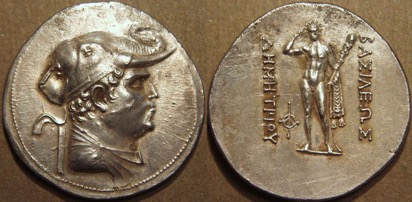
\includegraphics[width=.6\linewidth]{Raza-Figure01}
	\caption{Demetrius I. King wearing elephant headdress / Heracles holding diadem, club, and lion skin.
		{\normalfont\scriptsize \\ \coinindia}}
	\label{fig:Raza-Figure01}
\end{figure}
%\end{wrapfigure}

The first coin type under consideration is the elephant headdress.
This refers to obverse side designs representing the ruler in a headdress resembling an elephant's head.
Although three kings issued the coin type, discussion has centred on the coins of Demetrius I
(c. 200-185\BC) (see \cref{fig:Raza-Figure01}), the Graeco-Bactrian king who first invaded India \parencites[47--48]{Bopearachchi2011}[17--18]{Kalita1997}.
Explanations for the symbolic meaning of the elephant headdress draw mainly on Greek precedent. Originally, the elephant headdress had adorned posthumous Hellenistic representations of Alexander the Great, not unlike the lion skin of Heracles. It is thought that Alexander was being represented as an elephant slayer and that the headdress symbolically alluded to his conquests in India, the land of elephants to the Greeks \parencites[50]{Curtis2007}[335]{Green1993}[104--105]{MacDowall2007a}.
Consequently, the weight of analogy leads to the conclusion that Demetrius’ elephant headdress also commemorated his Indian conquests. If so, Demetrius’ coin type would support negative assessments of Greek engagement with local traditions. The elephant was a sacred animal for ancient Indians and the ascribed symbolism is analogous to the story of the Persian king Cambyses’ killing of the Apis Bull in Egypt \parencite[11--19]{Gupta1983}. Accordingly, it has been said that the symbolism was one of “massacre d’elephant,” representing conquest \parencite[492]{Widemann2009}.

However, the conquest interpretation is at odds with the chronology. Although dates for the Indian campaigns are unavailable, numismatists point out that Demetrius’ elephant headdress coins appear from the outset of his reign, before the new king would presumably have the chance to invade India \parencite[157]{Holt2012}.
Nevertheless, the presupposition that Demetrius was emulating Alexander has led to arguments to the contrary, all of which associate the elephant with India.
Principally, there is the suggestion that the elephant headdress coins indicate that Demetrius’ conquests took place before he became king, presumably as a general of his father Euthydemus I (c. 230-200\BC) \parencite[157]{Holt2012}.
Another is that if not alluding to conquests already made, the elephant headdress represented Demetrius as a ‘second Alexander’, and thus heralding an intention to conquer India in the future \parencites[190]{Sidky2000}[132]{Tarn1951}.
This paper argues against such proposals, instead suggesting that Demetrius’ elephant headdress represented a symbol of royal power accommodating various cultural groups.

First, the authority for Demetrius’ Indian campaigns is Strabo, who describes the conqueror as \enquote*{Δημήτριος ὁ Εὐθυδήμου υἱὸς τοῦ Βακτρίων βασιλέως},
‘Demetrius, son of Euthydemus, the king of the Bactrians’ (Strab. Geo. 11.11.1).
Some read the Greek to mean that Strabo was withholding the royal title from Demetrius, and that Euthydemus was king at this time \parencites[157]{Holt2012}[99]{MacDowall2007c}.
If so, Demetrius’ introduction of the elephant headdress coins might have alluded to his previous Indian conquests under Euthydemus.
However, Strabo’s syntax is structured around Demetrius, and the sentence should read that the latter was both Euthydemus’ son and king of Bactria. The traditional reading is indeed that Demetrius was the king mentioned in the text \parencite[144]{Tarn1951}.
Consequently, Strabo does not support the placing of Demetrius’ Indian campaigns under Euthydemus.

Second, it has been argued that a Greek inscription from Kuliab, Tajikistan, hailing Demetrius as \emph{Kallinikos}, ‘the Glorious Victor’, alludes to his Indian conquests under Euthydemus, the reigning king whom the inscription honours as \emph{Basileus Megiston}, ‘the Greatest of all Kings” \parencites[110]{Hollis2011}[125]{Holt2012}[104--105]{MacDowall2007a}[99]{MacDowall2007c}.
However, the inscription could have been alluding to victories claimed against Antiochus III, the Seleucid king who had unsuccessfully invaded Bactria during the reign of Euthydemus in 208-206\BC \parencite[48]{Bopearachchi2007}.
Polybius’ account of the war indicates that Demetrius was a young man, and thus old enough to have participated in some leading role (Pol. Hist. 11.34).
In addition, the wording of Euthydemus’ epithet suggests that the inscription is describing his successful resistance to Antiochus, who had adopted the title of \emph{Basileus Megas}, ‘the Great King’ \parencites[111]{Hollis2011}[125]{Holt2012}.
Thus, the Kuliab inscription does not necessarily suggest that Demetrius campaigned in India under Euthydemus.

Finally, while the dates cannot be fixed with any certainty, Graeco-Bactrian expansion into India seems improbable during the reign of Euthydemus.
Antiochus invaded India after the Bactrian war, evidently still ruled by independent kings such as Sophagasenus.
Meanwhile, nomads had begun troubling the Graeco-Bactrians, and Polybius writes that Euthydemus warned Antiochus of the mutual threat from an imminent invasion (Pol. Hist.11.34).
Significantly, the loss of Sogdiana – now mainly Tajikistan – coincided with the war with Antiochus, who seemed convinced to make peace with Euthydemus \parencites[38--39]{Holt1981}[135]{Holt1999}.
Euthydemus was probably preoccupied with the nomads for the remainder of his reign, and upon becoming king, Demetrius, too, might have been troubled by them.
Extensive fortification projects were initiated in the Sogdian frontiers of the kingdom beginning c. 200\BC, including new walls for the city of Ai Khanoum \parencites[38--39]{Holt1981}[135]{Holt1999}[60--61]{Lerner1999}[236]{Widemann2000}.
Accordingly, it is difficult to associate Demetrius’ elephant headdress chronologically with the Indian campaigns.
The coin type appeared from the outset of Demetrius’ reign, while the invasion of India took place sometime later.

Besides chronological difficulties, there are some stylistic differences that suggest Demetrius’ elephant headdress was not analogous to representations of Alexander, whose possible emulation underpins the conquest interpretation.
Mainly, Demetrius’ headdress is rendered as a military helmet, the rim being visible just above his hair and ear.
In addition, the elephant’s head is evidently animated, including an open eye and an upraised trunk in the saluting ‘S’ shape.
This suggests the vitality of the animal.
In contrast, Alexander was represented in an elephant skin draped around his head,
the lifelessness evident from the lack of eyes and a trunk lying flat in
a reverse ‘C’, or a ‘U’ lying down on its side \parencites[11]{Dahmen2007}[37]{Marcinkiewicz-Joseph2016}[48]{Maritz2004}[63]{Smith1986}.
The differences indicate Demetrius was not representing himself as an elephant slayer, and that the headdress need not necessarily be associated with conquests in India. 

In fact, the elephant was associated with the Graeco-Bactrian army, reflecting the animal’s prestigious status as a symbol of power in the Hellenistic world.
Graeco-Bactrian military \emph{phalarae}, metal disks worn as decorations by Graeco-Bactrian soldiers, represent war elephants prominently.
In addition, it is suggested that the Graeco-Bactrian infantrymen wore helmets modeled on the elephant’s head \parencites[170]{Abdullaev1995}[1206-1211]{Bannikov2013}[9--10]{Pfrommer1993}[588]{Treister1999}.
If so, royal self-presentation in elephant garb would be explicable in the context of Graeco-Bactrian military iconography, inspired by the Hellenistic tradition of war elephants.

The ‘animalisation’ of the monarch could have resonated locally as well. Animal headdresses were traditional in Bactria and it was believed that they transferred the power and attributes of animals to the wearer \parencite[215--226]{Lerner2009}.
Thus, Bactrians might have thought that Demetrius was symbolically claiming the strength of the elephant for himself, and that may have been the intention.
Self-aggrandisement of royal power through approximation to powerful animals was a recurring feature of Hellenistic kingship.
For example, Appian writes that horns adorning statues and images of Seleucus commemorated his supposed feat in taming a wild bull with his bare hands,
attesting to his bull-like strength \parentext{App. Syr. 57; \cites[53]{Alonso2014}[120]{Erickson2013}}.

Since certain animals were associated with divinities, their attributes could be considered divine tokens as well, ‘divinising’ symbols.
Thus, Libanius believed that Seleucus’ horns paid homage to the bull-goddess worshipped in his native Antioch, the Greek Io \parentext{\cites[121]{Erickson2013}; Lib. Or. 11.92}.
Significantly, elephant head crowns were a divinising symbol of the Indian sky god Indra, and worn by the south Indian Pallava kings consecrated as \emph{Narendra}, ‘the Indra of Man’ \parencite[66--70]{Hudson2008}.
Although the Pallavas are relatively late, elephants were a traditional symbol of kingship in India, and Justin records the story of an elephant consecrating Chandragupta Maurya – the Indian ruler who fought Seleucus – as king (Justin. Ep. 15.4).
Thus, Demetrius’ elephant headdress would not have necessarily given affront to his new subjects in India, who might have recognised royal power in the imagery \parencite[465]{Narain2003}.
Suggestively, the Indo-Greek Demetrius III (c.\,100\BC) later represented himself in an elephant headdress, deploying the thunderbolt – an attribute of Indra – as the reverse design \parencite[17--18]{Kalita1997}.  

Finally, it is notable that the reverse of Demetrius’ elephant headdress coin type depicts the coronation of Heracles, the demigod whom the Greeks tried to identify with local figures (see \cref{fig:Raza-Figure01}) \parencites[70--80]{Bukharin2004}[140]{Stanco2012}.
These include the ‘Bactrian Heracles’ mentioned by Arrian and the ‘Indian Heracles’ cited by Megasthenes, with both being known since the time of Alexander the Great \parentext{Arr. Anab. 4.28; Arr. Ind. 8.4}.
Thus, the coins draw attention to royal sovereignty, and perhaps in a cross-cultural context understood by local subjects.
Plutarch writes that the Bactrians worshipped Greek gods,
while Megasthenes adds that Indians worshipped Heracles \parentext{Arr. Ind. 8.4; Plut. Mor. 328d; \cite[420]{Potter2003}}.
It is argued that the material evidence supports the existence of a cult for Heracles in Bactria, and later, India as well \parencite[248]{Stanco2012}. 

Even if the local worship of Greek gods remained superficial, Plutarch and Megasthenes thought otherwise, which is possible if they identified local gods with Greek ones (\emph{interpretatio graeca}).
Significantly, Demetrius’ coins depicted the goddess Artemis with a radiate halo around the head, indicating her approximation to Anahita, the regal deity worshipped by the Bactrians in Ai Khanoum (see \cref{fig:Raza-Figure02})  \parencites[242]{MacDowall2007b}[420]{Potter2003}.
The resulting Artemis-Anahita appeared on the reverse side of coins with an obverse portrait of Heracles, suggesting that Demetrius’ self-presentation tried to take into account his various subjects.
Thus, the elephant headdress coin type can possibly be included amongst others that attempted to express royal power in a cross-cultural context.

\begin{figure}[!htb] %Figure 2
	%\begin{wrapfigure}{O}{0.5\textwidth} 
	\centering
	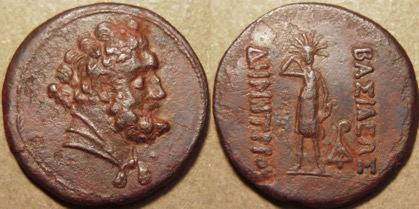
\includegraphics[width=.6\linewidth]{Raza-Figure02}
	\caption{Demetrius I. Bust of Heracles / Artemis with radiate halo. 
		{\normalfont\scriptsize \\ \coinindia}}
	\label{fig:Raza-Figure02}
\end{figure}
%\end{wrapfigure}

The next coin type under discussion is the ‘elephant aegis’.
This refers to an obverse portrait of the monarch wearing an elephant’s head on his left shoulder (see \cref{fig:Raza-Figure03}).
The coin type was issued solely by Lysias (c. 120-110\BC), an Indo-Greek king who ruled in modern Afghanistan and Pakistan \parencite[121]{Mairs2014}.
The design constitutes Lysias’ innovation on a standard obverse type in which Indo-Greek kings wore a protective goatskin aegis bearing the face of Medusa (see \cref{fig:Raza-Figure04}) \parencite[35]{Whitehead1970}.
One reading of the coin type is based on the elephant slayer motif. Lysias was the second king to wear an elephant headdress on coins, and just as with Demetrius I, it has been suggested that his coinage symbolises Indian conquests \parencites[341]{Cribb2011}[107]{Widemann2003}.
Certainly, the coin type represents Lysias in the act of hurling a spear, alluding to the Graeco-Macedonian concept of \emph{doriktetos chora}, ‘by the spear’, meaning the right of rule by conquest \parencite[27]{Billows1995}.
If this reading is correct, Lysias’ elephant head was a symbol of conquest, and not a traditional Greek aegis which imbued the wearer with the protection of Zeus and Athena \parencite[185]{Holt1999}.

\begin{figure}[!htb] %Figure 3
	%\begin{wrapfigure}{O}{0.5\textwidth} 
	\centering
	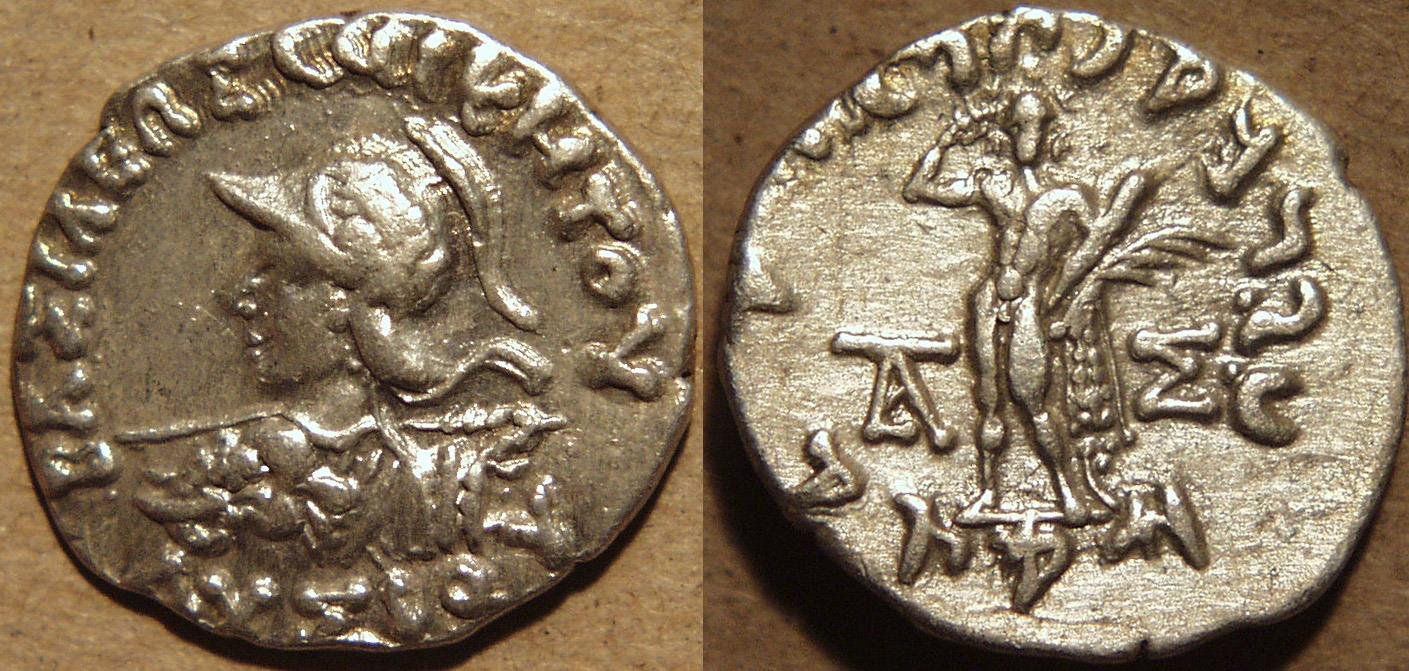
\includegraphics[width=.6\linewidth]{Raza-Figure03}
	\caption{Lysias. King brandishing spear and wearing an elephant’s head with protruding tusks on left shoulder / Heracles holding diadem, club, and lion skin. 
		{\normalfont\scriptsize \\ \coinindia}}
	\label{fig:Raza-Figure03}
\end{figure}
%\end{wrapfigure}

On the other hand, it has been pointed out that Lysias wears the elephant’s head, “as if it belonged to an aegis” \parencite[86]{Bopearachchi1990}.
Furthermore, the kings wearing the goatskin also represented themselves hurling spears, making the spear-thrower motif a general symbol of royal power (see \cref{fig:Raza-Figure04}).
Thus, some suggest that Lysias’ elephant head did constitute an aegis, albeit one that represented him as a warrior-king under the protection of an unspecified ‘Indian elephant deity’ \parencite[35]{Whitehead1970}.
This view holds that there was a divide between Greek and Indian religions, and that Lysias presumably adhered to the ‘elephant party’ of Indo-Greeks that rejected Greek religion, warring with the traditionalists from the ‘Zeus party’ \parencites[94]{Whitehead1970}[26]{Widemann2007}.

\begin{figure}[!htb] %Figure 4
	%\begin{wrapfigure}{O}{0.5\textwidth} 
	\centering
	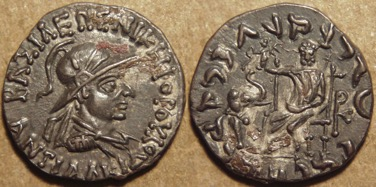
\includegraphics[width=.6\linewidth]{Raza-Figure04}
	\caption{Antialcidas. King brandishing spear and wearing goatskin aegis on left shoulder / Zeus with an elephant. Nike on top of an elephant’s head.
		{\normalfont\scriptsize \\ \coinindia}}
	\label{fig:Raza-Figure04}
\end{figure}
%\end{wrapfigure}
 
Some have emphasised the superficial nature of the ‘elephant party’, suggesting that the force of Lysias’ symbolism lay in its oppositional value \parencite[114]{Widemann2003}.
There had been no intentional concession to Indian cults. Lysias merely subverted a traditional Greek iconographic scheme, and thereby disassociated himself from the ‘Zeus party’, which evidently attempted to enforce Indian worship of Greek gods \parencite[26]{Widemann2007}.
This paper supports the view that Lysias’ elephant’s head represented an aegis meant to imbue the king with divine protection and power.
However, the paper argues against the existence of a gulf between Greek and Indian cults, suggesting that Lysias was expressing his royal power in a cross-cultural context that accommodated both groups.
  
First, Lysias was possibly co-ruler with another Indo-Greek king, Antialcidas (c. 115-95\BC) \parencite[121]{Mairs2014}.
Both were contemporaries who ruled in the roughly same area, and shared monograms – the identifying marks made on coins by minting officials.
This suggests that they both had access to the same mints at the same time.
In addition, Lysias and Antialcidas evidently issued joint coins, which bear legends or inscriptions of both kings.
One coin type features the legend of Lysias on the obverse side, and that of Antialcidas on the reverse, while another reverses the arrangements of the first.
The existence of two antithetical hybrid issues suggests that the coins were part of a deliberate series, and not erroneous issues, as some had supposed before the discovery of the second specimen \parencites[1184]{Bopearachchi2015}[154]{Narain2003}.
If it is accepted that the hybrid coins were jointly issued, Lysias and Antialcidas were probably co-rulers, and their coins cannot be studied without reference to each other.

The significance of Lysias’ association with Antialcidas is that the latter represented the elephant in proximity to Greek divinities.
One reverse design features Zeus, holding a sceptre, and striding beside an elephant. Meanwhile, the goddess Nike, holding a wreath symbolising victory, stands on top of the elephant’s head (see \cref{fig:Raza-Figure04}) \parencite[27]{Narain1991}.
Another reverse design depicts the protome of an elephant, its trunk raised like a salute to the enthroned Zeus.
In turn, Zeus holds a sceptre in one hand and, with the other, supports a wreath-bearing Nike symbolising victory (see \cref{fig:Raza-Figure05}) \parencite[33--34]{Whitehead1970}.
Significantly, the obverse of the first specimen represents Antialcidas in the goatskin aegis eschewed by Lysias.
Antialcidas thus might have been invoking the power and protection of Zeus, who also has the elephant under his aegis on the coins. 

\begin{figure}[!htb] %Figure 5
	%\begin{wrapfigure}{O}{0.5\textwidth} 
	\centering
	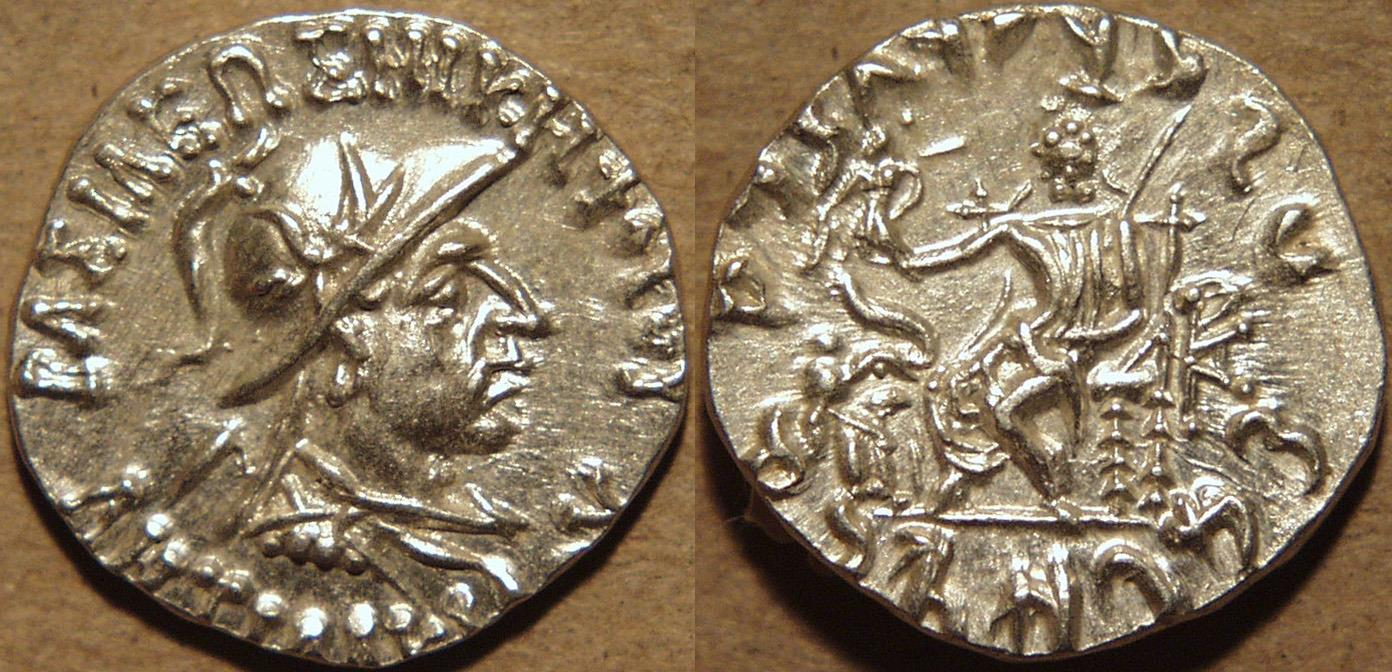
\includegraphics[width=.6\linewidth]{Raza-Figure05}
	\caption{Antialcidas. Portrait of king / Elephant saluting Zeus on throne. Nike in Zeus’ right hand.
		{\normalfont\scriptsize \\ \coinindia}}
	\label{fig:Raza-Figure05}
\end{figure}
%\end{wrapfigure}

If Lysias and Antialcidas were co-rulers, it would be difficult to reconcile the high status accorded to the elephant on the one hand, and the predatory meaning ascribed to the elephant imagery on the other.
Accordingly, it is plausible that Lysias’ elephant’s head represents an innovation on the traditional aegis iconography, rendered in an Indian context with the elephant as a divinising symbol of Zeus.
An elephant’s head was not necessarily an affront to Indians. The elephant head crown of the Pallavas has been noted previously \parencite[66--70]{Hudson2008}. 
Moreover, although the elephant was the sacred animal of Indra, it had been evidently transferred to Zeus.
It is possible that elephant aegis originated as a result.
Notably, the \emph{Vedas} described Indra as being “clothed in might like an elephant”, suggesting a possible Indian tradition accessible to the Greeks and deployed in the context of Zeus \parencite[22]{Gupta1983}. 

In fact, Zeus himself might have been approximated to Indra.
It is suggestive that Antialcidas’ coins represent Zeus wielding a thunderbolt and in proximity to elephants, not unlike Indra’s representation in Indian tradition (see \cref{fig:Raza-Figure04,fig:Raza-Figure05,fig:Raza-Figure06}) \parencite[242--247]{MacDowall2007b}.
Similarly, the Graeco-Bactrian king, Antimachus I (c. 174-165\BC), associated the elephant and the thunderbolt on his coins (see \cref{fig:Raza-Figure07}). 

\begin{figure}[!htb] %Figure 6
	%\begin{wrapfigure}{O}{0.5\textwidth} 
	\centering
	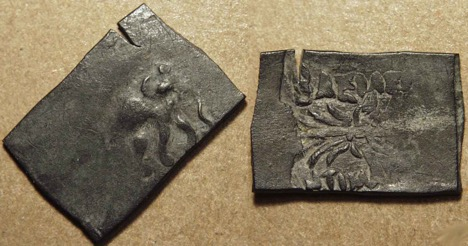
\includegraphics[width=.6\linewidth]{Raza-Figure06}
	\caption{Antialcidas. Zeus holding thunderbolt / Caps and palms of the Dioscuri.
		{\normalfont\scriptsize \\ \coinindia}}
	\label{fig:Raza-Figure06}
\end{figure}
%\end{wrapfigure}

\begin{figure}[!htb] %Figure 7
	%\begin{wrapfigure}{O}{0.5\textwidth} 
	\centering
	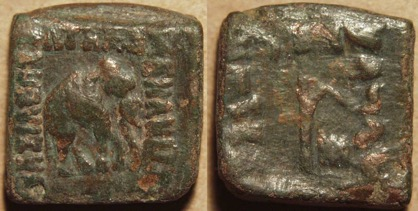
\includegraphics[width=.6\linewidth]{Raza-Figure07}
	\caption{Antimachus I. Elephant walking right / Winged thunderbolt.
		{\normalfont\scriptsize \\ \coinindia}}
	\label{fig:Raza-Figure07}
\end{figure}
%\end{wrapfigure}

Finally, there is the evidence of Heliodorus, the ambassador of Antialcidas to the court of the Indian king, Bhagabadra, in Vidisha.
While in Vidisha, Heliodorus left behind an inscription professing devotion to Vasudeva, a manifestation of the god Vishnu.
Significantly, Heliodorus designated the pillar on which the inscription was written as the ‘Garuda pillar’, alluding to the sacred hawk of Vishnu.
It is thought that the structure was originally topped by a statue of Garuda \parencite[126--127]{Mairs2014}.
Thus, it seems the Indo-Greeks took part in local cults, and were aware of the iconographic schemes of local gods, including possibly the elephant’s proximity to Indra.
Accordingly, Indra might have been worshipped as Zeus, accounting for the Greek aegis rendered in an Indian context.
If so, this suggests a royal conception of power that extended beyond their Greek heritage, incorporating local Indian traditions as well.

The last coin type under discussion is the ‘elephant goad’.
This refers to coins with an elephant on the obverse side and an elephant goad on the reverse – the goad being the tool used by Indian \emph{mahouts} or elephant drivers to train and control the animal (see \cref{fig:Raza-Figure08}).
The coin type was issued by only one Indo-Greek king, Menander I (c. 165/155-135\BC), whose kingdom was centred on the Punjab in modern Pakistan and India.
Menander was an important ruler whose reputation has been preserved in both Indian and classical sources \parencite[14--17]{Bopearachchi1993}.
The Buddhist text \emph{Milindapanha} portrays Menander as a wise Buddhist king who abdicated his throne to retire to an ascetic life \parencite[14--17]{Bopearachchi1993}.
Classical authors provide a different perspective.
Plutarch writes that Menander was celebrated for his rule, but that he died in camp, presumably while on a military campaign.
Strabo adds that Menander was the most successful Indo-Greek general, comparing him to Alexander the Great \parentext{\cite[180--183]{Holt1999}; Strab. Geo. 11.11.1; Plut. Mor. 821d}.

\begin{figure}[!htb] %Figure 8
	%\begin{wrapfigure}{O}{0.5\textwidth} 
	\centering
	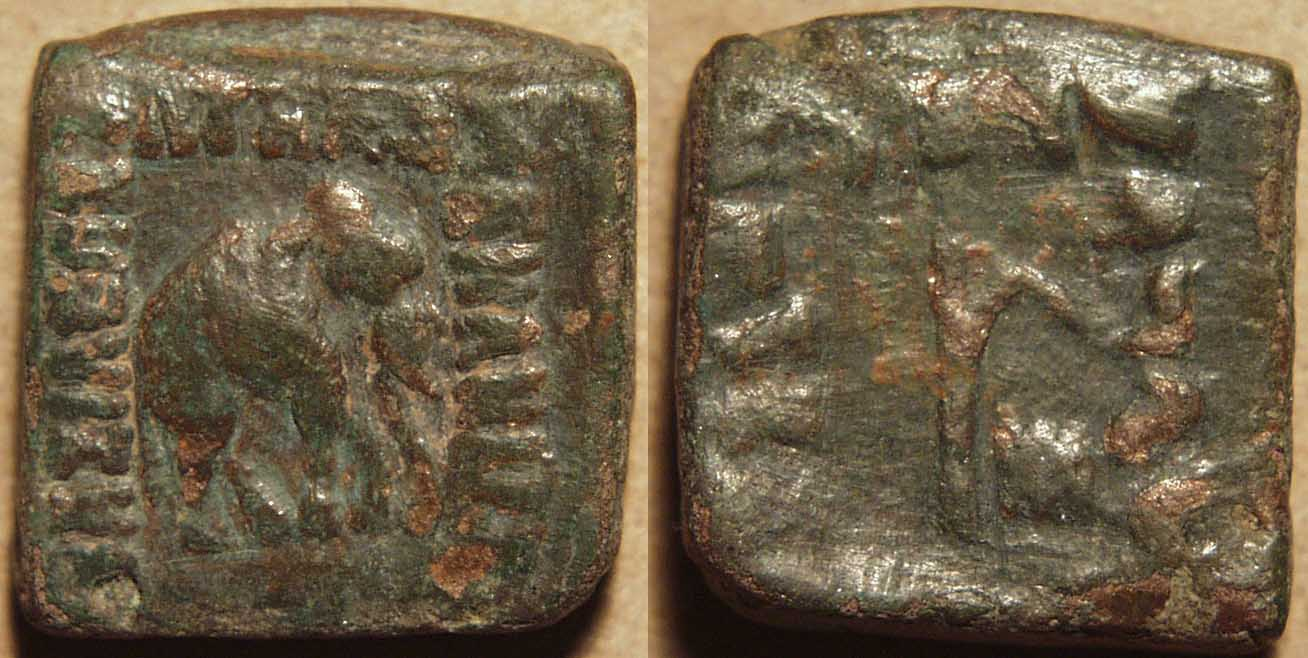
\includegraphics[width=.6\linewidth]{Raza-Figure08}
	\caption{Menander I. Elephant walking right / Elephant goad.
		{\normalfont\scriptsize \\ \coinindia}}
	\label{fig:Raza-Figure08}
\end{figure}
%\end{wrapfigure}

In scholarship, the testimony of the classical authors has been privileged by some, and Menander is considered primarily as a Hellenistic warrior king.
One scholar thus observes that, “true to form” of a Hellenistic king, Menander had died waging war.
Menander is also associated with Eucratides I (c. 170-145\BC),
the Graeco-Bactrian king, who, according to Justin,
had weakened himself through the waging of incessant wars,
but in more cynical translations was said to have “bled Bactria to death”
\parentext{\cites[128]{Holt2005}[156]{Mairs2014}[270]{Tarn1951}; Justin. Ep. 41.6}.
In contrast, Menander’s representation as a philosopher king in the \emph{Milindapanha} has been summarily dismissed as Buddhist missionary ‘propaganda’, which overlooks his actual ‘warlike’ and ‘murderous’ tendencies \parencites[234]{Widemann2000}[15--16]{Widemann2007}.
Accordingly, the elephant and goad on Menander’s coins have been associated with Greek imperialism, presumably representing the Greeks as the masters of elephants, and hence of Indians \parencite[87--89]{Fussman1993}.
This paper argues that this was not necessarily the case and that Menander’s coin type might have represented royal power in a cross-cultural context, accommodating both Greeks and Indians.

While the \emph{Milindapanha} might betray a Buddhist bias, it is suggestive that Menander was considered an ideal figure to represent Indian ideas of kingship.
Significantly, Plutarch writes that after Menander’s death, his subjects competed over his mortal remains and divided them as relics for internment in various monuments.
This calls to mind the division of the Buddha’s ashes in \emph{stupas}, ‘tombs’ set up by his followers, and indicates that Menander might have been honoured by his Indian subjects in the Buddhist fashion \parentext{Plut. Mor. 821d; \cite[145]{Rothkrug2006}}.
Regardless of whether or not Menander was a convert, it seems that Buddhists remembered him with esteem, and honoured him as one of their own \parencite[644]{Mairs2015}.
Thus, Menander might have conceivably reached out to his Indian subjects. The coin type with the elephant and the goad might have been one such instance.

First, elephants had more than just a military role in Indian political tradition.
Owing to their fondness for bathing and the use of the trunk to spray water, elephants became associated with fertility and sky divinities such as Indra, and attributed rainmaking powers \parencite[19]{Gupta1983}.
One origin story was that elephants were clouds cursed to wander among humans, and thus responsible for rainfall when their brethren would bear down on the earth for conjugal visits.
Indian kings were therefore required to maintain royal elephants known as the ‘king’s clouds’ to ensure rainfall for the kingdom’s prosperity.
In fact, elephants were one of the seven \emph{ratnas}, or 'jewels', the necessary symbols of a legitimate Indian monarch \parencites[38--39]{Gonda1966}[107]{Campbell2015}.
As a young ruler, the Buddha charitably gave away the royal elephant to a neighbouring kingdom suffering from drought but, in turn, invited thirst and famine on his own subjects who eventually drove him from his throne \parencite[23--24]{Gupta1983}.
Consequently, the goad might have signified Menander’s possession of elephants, and hence an acknowledgment of his royal duty to maintain the fertility and abundance of the kingdom.

Second, the elephant and goad may have had connotations of justice.
The purposes of the goad were to tame, control, and direct the elephant \parencite[66--67]{Trautmann2015}.
The symbolic nature of the goad as an instrument of control consequently led to its association with law. \emph{Nirankusa}, ‘unrestrained’, the antonym derived from \emph{ankusa}, ‘restrain’, the word for goad in Sanskrit, referred to those who did not follow social norms and rules.
Accordingly, the elephant-headed god Ganesha, who possibly originated during the Indo-Greek period, held the goad as a symbol of his power to restrain the forces of evil \parencites[96]{Alter2004}[144]{Dhavalikar1981}.
Similarly, Buddhist tradition compared the love and wisdom of the Buddha to the goad, capable of taming the wickedness of the elephant Nalagiri \parencite[96]{Dhammika2005}.
Thus, Menander might have been alluding to his role in upholding justice for his subjects, in addition to supporting their welfare.
This reading of the coins would support Menander’s engagement with local traditions and practices of kingship, and possibly account for his reception in Indian tradition.
Notably, Menander did strike coins showing the \emph{chakra}, the ‘wheel’, the symbol par excellence of the \emph{Chakravartin}, the rightful universal monarch of Indian tradition (see \cref{fig:Raza-Figure09}) \parencite[15]{Stanco2012}.

\begin{figure}[!htb] %Figure 9
	%\begin{wrapfigure}{O}{0.5\textwidth} 
	\centering
	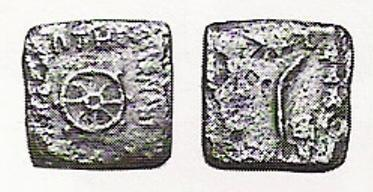
\includegraphics[width=.6\linewidth]{Raza-Figure09}
	\caption{Menander I. Wheel / Palm branch.
		{\normalfont\scriptsize \\ \coinindia}}
	\label{fig:Raza-Figure09}
\end{figure}
%\end{wrapfigure}

Finally, the elephant and goad coins might have represented Menander’s military power, which is emphasised by classical authors \parencite[644]{Mairs2015}.
For the Greeks, a goad represented power over elephants and symbolically alluded to the strength of the wielder.
Alexander had evidently aggrandised his Indian triumphs on the so-called ‘elephant medallion’ coins by representing his defeat of the Indian ruler, Porus, a giant figure controlling an elephant with a goad \parencites[151--152]{Holt2003}[204--205]{Stewart1993}.
While Menander did not represent himself as an elephant tamer per se, the goad might have nevertheless represented royal military power to Greeks, as evident in the king’s possession of powerful war elephants. 

Moreover, the Greek author of the \emph{Periplus Maris Erythrae} reports seeing the coins of Menander in the Indian port of Barygaza (Baruch), and takes special note of the iconography \parentext{PME. 47}.
Conceivably, the author would have interpreted the coins in a Greek context. In contrast, an Indian might have equated the elephant and the goad with local traditions.
The point is that the coin type would have resonated in both a Greek and an Indian context.
Consequently, it would be unjustified to dismiss Menander’s reputation as an Indian philosopher king, and focus on the Hellenistic warrior king found in the classical authors.
Menander could have represented himself as both, appealing to Greeks and Indians.

In conclusion, elephant motifs on Graeco-Bactrian and Indo-Greek coinage legitimised royal authority in a cross-cultural context.
The view that the Graeco-Bactrian and Indo-Greek kings did not engage with local ruling traditions is not borne out by the coins.
The picture that emerges supports the recent literature emphasising the cosmopolitan conception of royal power in the Hellenistic kingdoms \parencite[11]{Strootman2014}.
However, a ‘Hellenocentric’ approach has meant that the cross-cultural significance of the elephant motifs is not fully appreciated.
When studying the coins, scholars should take note to consider not only the Greek context, but also the possible local significance of the iconography.
Through consideration of local contexts, scholars will be able to gain a better understanding of how Hellenistic kings established and maintained their power over diverse, multi-ethnic populations.

\IJSRAseparator
I \IJSRAsection{Acknowledgements} would like to thank the IJSRA editors and Candida Crewe for their assistance and critical comments.
\IJSRAclosing%<<<< DO NOT change this line
\end{document}